\documentclass[11pt,a4paper,ngerman]{article}
\usepackage[bottom=2.5cm,top=2.5cm]{geometry} 
\usepackage{babel}
\usepackage[utf8]{inputenc} 
\usepackage[T1]{fontenc} 
\usepackage{ae} 
\usepackage{amssymb} 
\usepackage{amsmath}
\usepackage{amsthm} 
\usepackage{graphicx}
\usepackage{fancyhdr}
\usepackage{caption}
\usepackage{subcaption}
\usepackage{fancyref}
\usepackage{enumerate}
\usepackage{listings}
\usepackage{xcolor}
\usepackage{paralist}
\usepackage{tabularx}

\usepackage[pdftex, bookmarks=false, pdfstartview={FitH}, linkbordercolor=white]{hyperref}
\usepackage{fancyhdr}
\pagestyle{fancy}
\fancyhead[C]{Numerik I}
\fancyhead[L]{Übung 7}
\fancyhead[R]{SoSe 2013}
\fancyfoot{}
\fancyfoot[L]{}
\fancyfoot[C]{\thepage \hspace{1px} of \pageref{LastPage}}
\renewcommand{\footrulewidth}{0.5pt}
\renewcommand{\headrulewidth}{0.5pt}
\setlength{\parindent}{0pt} 
\setlength{\headheight}{0pt}

\date{Tutor: Christina Schulz}
\title{Übung 7}
\author{Max Wisniewski, Alexander Steen}


%%
%% Enviroments for proofs and lemmas
%%
\newtheorem{lemma}{\bfseries Claim}

\begin{document}

\lstset{language=Pascal, basicstyle=\ttfamily\fontsize{10pt}{10pt}\selectfont\upshape, commentstyle=\rmfamily\slshape, keywordstyle=\rmfamily\bfseries, breaklines=true, frame=single, xleftmargin=3mm, xrightmargin=3mm, tabsize=2, mathescape=true}

\renewcommand{\figurename}{Figure}

\maketitle
\thispagestyle{fancy}

%%%%%%%%%%%%%%%%%%%%%%%%%%%%%%
%% Aufgabe 1     %%%%%%%%%%%%%%%%
%%%%%%%%%%%%%%%%%%%%%%%%%%%%%%
\subsection*{Aufgabe 1}

\subsubsection*{(a)}

Gegeben sei das Integral $J$ mit folgender (exakter) Lösung:
\begin{equation*}
    J := \int_0^1 \sin(\pi x) \, dx = \frac{2}{\pi}
\end{equation*}

Nach Skript ist der Fehler bei summierter Trapezregel beschränkt durch $h^2 \|f^{(2)} \|_\infty$ und damit für uns gegeben durch

\begin{equation*}\begin{array}{crcl}
    & h^2 \| f^{(a)} \|_\infty &<& 10^{-4}\\
\Leftrightarrow & \frac{1}{n}^2 \| -\pi^2 \sin (\pi x) \|_\infty &<& 10^{-4}\\
\Leftrightarrow & \frac{pi}{n}^2 &<& 10^{-4}\\
\Leftrightarrow & n &>& 100 \pi
\end{array}\end{equation*}

Nun müssen wir nach der Formel
$$
    I_\Delta (f) = \overset{m}{\underset{k=1}{\sum}} \overset{n}{\underset{i=0}{\sum}} \lambda_{ik} f(x_{ik}) h_k
$$
die Funktion insgesammt $2n$ mal auswerten oder aber, da sich die Werte immer überschneiden, müssen wir sie nur $n$ mal berechnen
und uns den letzten Wert für das nächste Trapez merken.

\subsubsection*{(b)}

Gegeben ist das Integral $\int_0^1 f(x) dx$ und die Knoten $x_0 = 0, x_1 = \frac{1}{4}, x_2 = 1$.
Bestimmen Sie die Quadraturformel mit Ordnung 3.\\

\textbf{Lösung:}\\
%Die Quadraturformel mit Ordnung 3 ist nach Newton-Côtes Formel die simpsonregel. Da wir nur 3 Punkte haben, betrachten wir
%nur dieses Interval.\\
%
%\begin{equation*}\begin{split}
%    I_\Delta (f) &= \overset{2}{\underset{i=0}{\sum}} \lambda_{i} f(x_i) h_{i}\\
%    &= \frac{f(0)}{6} + \frac{4 \cdot f(\frac{1}{4})}{6} + \frac{f(1)}{6}
%\end{split}\end{equation*}
%
%Äh, ich glaub man sollte noch 3 Punkte in die beiden Intervalle je setzten....
%ICH glaube: Newton-cote kann man hier nicht verwenden, da kein äquidistanter gitter.
%-> selber quadraturformel aufstellen. \\
%
Gegeben ist das Gitter $\Delta = \{x_0 < x_1 < x_2 \} = \{0, \frac{1}{4}, 1 \}$.
Die Quadraturformel dritter Ordnung $I_2(f)$ (also Interpolationspolynomgrad 2)
erhält man durch Interpolation des Integranden durch ein Polynom $p_2$ vom Grad 2.
Setzt man nun die Legendre-Darstellung des Polynoms $p_2 = \sum_{k=0}^2 f(x_k)L_k$ ein,
erhält man als Quadraturformel

\begin{equation*}\begin{split}
I_2(f) &= \int_0^1 p_2(x) dx \\
       &= \sum_{k=0}^2 f(x_k) \lambda_k
\end{split}\end{equation*}

Die Gewichte $\lambda_k$ können (wie z.B. im CoMa II gelernt) durch die Vorschrift

\begin{equation*}
  \lambda_k = \int_0^1 L_k(x) dx
  \quad \quad
  L_k(x) = \prod_{j=0,j \neq k}^2 \frac{x-x_k}{x_j - x_k},
  k = 0, 1,2
\end{equation*}

berechnet werden.
Einsetzen ergibt:
\begin{center}
\begin{tabular}{c|c|c}
k & $L_k(x)$ & $\lambda_k$ \\
\hline \hline
0 & $x(4x -5)+1$ & $-\frac{1}{6}$\\
1 & $-\frac{16}{3} (x-1) x$ & $\frac{8}{9}$ \\
2 & $\frac{1}{3}x (4x -1)$ & $\frac{5}{18}$\\
\end{tabular}
\end{center}
und damit

\begin{equation*}
I_2(f) = -\frac{1}{6} f(x_0) + \frac{8}{9} f(x_1) + \frac{5}{18} f(x_2)
\end{equation*}
%%%%%%%%%%%%%%%%%%%%%%%%%%%%%%
%% Aufgabe 2                           %%%%%%%%%%%%%%%%
%%%%%%%%%%%%%%%%%%%%%%%%%%%%%%
\subsection*{Aufgabe 2}
Es sollen zwei Programme zur berechnung von
$$
    \int_a^b f(x) dx
$$
geschriebe werden.

Die folgenden matlab-Programme rechnet die jeweiligen Newton-Cotes-Formeln aus. Der Aufwand ist jeweils auf die Berechnung des Programms bezogen, welche Funktionsauswertungen nicht mehrfach benutzt und darum etwas ineffizienter ist, als es sein könnte.

\subsubsection*{(a)}
Schreiben Sie eine Funktion zur Berechnung mit summierter Trapezregel.\\

\textbf{Lösung:}\\
\begin{lstlisting}[language=matlab,numbers=left,caption=Quadratur nach Trapez-Regel]
function [S] = trapQuad(a,b,f,n)
% Gibt den Zahlenwert S der Quadratur zurueck
%
% [a,b] Integrationsintervall
% f zu intigrierende Funktion
% n anzahl der teilintervalle

ab = [a,b];
% Bezeichnungen ab hier wie im Skript
% h ist der Abstand zwischen den Stellen
h = (ab(2) - ab(1))/n;
% z sind die Stuetzstellen
z = ab(1) + (1:n).*h;

% Gewichte jeweils aus dem Skript entnommen,
% sowie Berechnungsvorgehen

%% Trapez-Berechnungsvorschrift
x = @(k) z(k);
S = h/2 * (f(ab(1)) + f(ab(2)));
for k = 2:(n),
   S = S + h*f(x(k)); % Siehe Skript
end
return % Aufwand n+1
\end{lstlisting}

\subsubsection*{(b)}
Schreibe Sie eine Funktion zur Berechnung mit summierter Simpsonregel.\\

\textbf{Lösung:}\\
\begin{lstlisting}[language=matlab,numbers=left,caption=Quadratur nach Simpson-Regel]
function [S] = simpQuad(a,b,f,n)
% Gibt den Zahlenwert S der Quadratur zurueck.
%
% [a,b] Integrationsintervall
% f zu intigrierende Funktion
% n anzahl der teilintervalle

ab = [a,b];
%% Simpson-Berechnungsvorschrift
% (Algorithmisches) Vorgehen analog zu Trapez
x = @(k,j) z(k/2) + j*h/2;
S = 0;
for k = 1:(n),
   S = S + h/6 * (f(x(2*k,0)) + 4*f(x(2*k,1)) + f(x(2*k,2)));
end
return % Aufwand 3n
\end{lstlisting}

\subsubsection*{(c)}
Testen Sie die Funktionen und beurteilen Sie die beobachtete Konvergenzordnungen.\\

\textbf{Lösung:}\\
Wir wählen als Funktion zum Testen $f = \sin(x)$. Diese Funktion ist glatt und beschreibt einen
gleichmäßigen Bogen, eignet sich also relativ gut für Quadraturen mit äquidistanten Stützstellen.


Die Auswertung der matlab-Funktionen aus a) und b) wurde mit folgendem Code gemacht:
\begin{lstlisting}[language=matlab]
>> for k = 1:50,                         
erg(k) = trapQuad(0,pi,f,6*k);
end
>> for k = 1:50,              
erg2(k) = trapQuad(0,pi,f,6*k);
end
\end{lstlisting}

Und dann mit diesem Code geplottet (Achsenbenennung weggelassen):
\begin{lstlisting}[language=matlab]
h=loglog(6:6:6*50,abs(2-erg)) 
h2=loglog(6:6:6*50,abs(2-erg2)) 
\end{lstlisting}
Dies kann man machen, da die exakte Lösung gegeben ist durch $\int_0^{\pi} \sin(x) \, dx = 2$.

\begin{figure}[ht]
\centering
\begin{subfigure}{0.45\textwidth}
	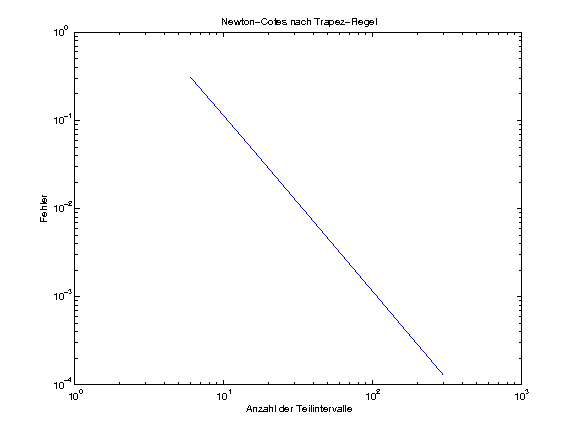
\includegraphics[width=\textwidth]{trapez.png}
  \caption{Fehler der Trapezregel}
\end{subfigure}
\begin{subfigure}{0.45\textwidth}
	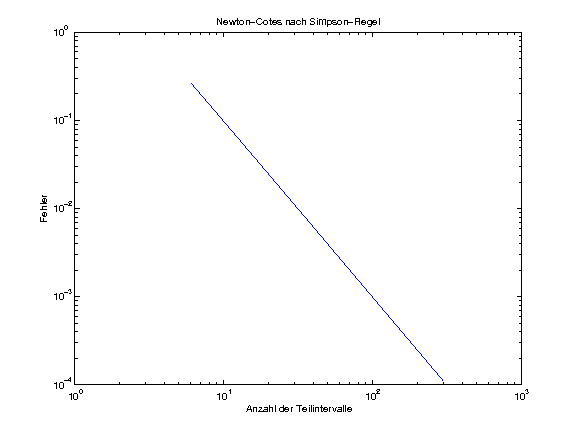
\includegraphics[width=\textwidth]{simpson.png}
  \caption{Fehler der Simpsonregel}
\end{subfigure}
\caption{Fehler der Newton-Cotes-Formeln (Aufgabe 2c)}
\end{figure}

Der lineare Verlauf (auf der log-Skala) der Fehler über die Teilintervalle zeigt ein akzeptables Verhältnis und ist bei beiden Formeln (nahezu) gleich. Die Steigung der Fehlerkurve auf der log-Skala zeigt die
gewünschte Konvergenzordnung.

%%%%%%%%%%%%%%%%%%%%%%%%%%%%%%
%% Aufgabe 3   %%%%%%%%%%%%%%%%
%%%%%%%%%%%%%%%%%%%%%%%%%%%%%%
\subsection*{Aufgabe 3}

Gewinnung einer Quadraturformel in höheren Dimensionen.

\subsubsection*{(a)}
Wie sieht die Interpolation auf einem Dreieck mit den Ecken $e_1 = (0,0), e_2 = (a,0), e_3 = (0,b)$ aus?\\

\textbf{Lösung:}\\
Als lineare Interpolation für $f(p)$ einen Punkt $p$ im Dreieck $T$ mit Eckpunkten $e_1, e_2, e_3$ können wir
$p$ als Linearkombination der Eckpunkte darstellen und dies als Gewichtung der Stützstellenauswertung benutzen.
Es gilt $p = (0,0) + s \cdot (a,0) + t \cdot (0,b)$ für $s,t \geq 0, s + t \leq 1$ und damit als Interpolation
$f(p) = f(0,0) + s \cdot f(a,0) + t \cdot f(0,b)$.

\subsubsection*{(b)}
Gewinnen Sie eine Quadraturformel für das Dreieck durch Integration der Lagrange-Polynome, gegeben
durch $L_k(e_i) = \delta_{ki}$.\\

\textbf{Lösung:}\\
tbd

\subsubsection*{(c)}
Leiten Sie die Formel für das Recheck her.\\

\textbf{Lösung:}\\
tbd


\label{LastPage}
\end{document}
